% Transcribed from Section_6_Differential_Equations(4).pptx.

\setcounter{section}{5}
\section{Differential Equations}
\begin{ILOssec}
\item \ILOg
\end{ILOssec}

% Source slide 2

\subsection{Introduction to differential equations}
\label{sec:ode_intro}

\begin{learningoutcomes}
\item Distinguish an ordinary differential equation from other types of differential equation and identify its order
\item Test whether an expression is a solution to an ODE and identify if it is a general or particular solution
\end{learningoutcomes}

% Source slide 3

\textbf{Examples in chemical reactions}

Consider a simple unimolecular reaction,
\[
A\to \text{products}
\]

The amount of species A left in the reaction is given by
\begin{align}
    \label{eq:unimol} \der{A}{t}=-kA \, ,
\end{align}
where $A$ is the amount of A, $k$ is the reaction rate constant, and $t$ is time.

Equation \eqref{eq:unimol} is an example of a `differential equation'. It cannot be simply integrated as the right-hand side involves the unknown function $A(t)$. The reaction rate is $kA$, \textit{i.e.} it is proportional to the amount of A. The reaction also uses up the species A and so the reaction rate determines the rate at which A is lost. Therefore, the rate of change of species A, $\der{A}{t}$, is equal to the negative of the reaction rate, $-kA$.

% Source slide 5

Now, consider a simple bimolecular reaction between gases
\[
A+B\to \text{products}
\]
where $A(t)$ and $B(t)$ are the concentrations of A and B respectively. The reaction rate depends on the concentrations of A and B and so the concentration of species A (assuming fixed volume) changes as
\[
\der{A}{t}=-{k}_{AB}AB \, .
\]
If the reaction starts with concentrations $A={A}_{0}$ and $B={B}_{0}$, then at time $t$, the same number of A and B molecules will be used up, so ${A}_{0}-A={B}_{0}-B$, and hence $B={B}_{0}+A-{A}_{0}$.

Therefore, the reaction rate is now a quadratic function of $A$
\[
\der{A}{t}=-{k}_{AB}A({B}_{0}+A-{A}_{0})
\]

It is possible the reaction rate may be even more complicated. It may also depend on temperature, which may depend simply on time or even on the reaction itself, e.g.
\[
\der{A}{t}=-{k}_{AB}(t)A({B}_{0}+A-{A}_{0})
\]

% Source slide 7

\textbf{Ordinary differential equations (ODEs)}

An ordinary differential equation (ODE) is an equation linking a variable (say $t$), a function (say $y$) and its derivatives $\der{y}{t}$, $\der{^2y}{t^2}$, etc.
\[
f\left(t,y,\der{y}{t},\der{^2y}{t^2},\ldots \right)=0
\]

The term ``ordinary'' distinguishes this from other types of differential equation, such as partial differential equations (where the functions depend on more than one variable). We will only consider ODEs in this course.

% Source slide 8

\textbf{Order of Differential Equations.}

The highest derivative present determines the order of the differential equation.
\begin{itemize}
\item A first-order equation is of the form
\[
f_1\left(t,y,\der{y}{t}\right)=0 \, ,
\]
for example, $\der{A}{t}=-kA$ .
\item A second-order equation is of the form
\[
f_2\left(t,y,\der{y}{t},\der{^2y}{t^2}\right)=0\, ,
\]
for example, $\der{^2A}{t^2}=-m^2A$.
\end{itemize}
We will focus on first and second order ODEs in this course.

% Source slide 9

\goodbreak
\begin{example}[Lecture]
\label{ex:611}
Find the order of the following ODEs.
\begin{enumerate}[label=(\alph*)]
\item $\displaystyle \der{y}{x}=1+x^2y^2$\par
\item $\displaystyle \der{^2y}{t^2}=-ky$\par
\item $\displaystyle \left(\der{^3z}{t^3}\right)^7+\left(\der{^5z}{t^5}\right)^4=z^{12}$\par
\end{enumerate}
\end{example}
\begin{solution}
\begin{enumerate}[label=(\alph*)]
\item 1st order
\item 2nd order 
\item 5th order
\end{enumerate}
\end{solution}

% Source slide 13

\textbf{Solutions to differential equations.}

To `solve' a differential equation, e.g.
\[
{f}_{1}\left(t,y,\der{y}{t}\right)=0
\]
we need to write it in a form without the derivative (preferably in explicit form), e.g. $g\left(y,t\right)=0$ or preferably $y=h(t)$.

% Source slide 14

Consider the differential equation
\[
\der{y}{x}=xy
\]
It can be seen that $y=\exp ({x}^{2}/2)$ is a solution. Using the chain rule gives
\begin{align*}
\der{y}{x}&=x{e}^{\frac{{x}^{2}}{2}}
\\[4pt]
&=xy
\end{align*}
However, we also see that $\displaystyle y=5\exp ({x}^{2}/2)$ is a solution, since $\displaystyle \der{y}{x}=5x{e}^{\frac{{x}^{2}}{2}}$ and $\displaystyle xy=5x{e}^{\frac{{x}^{2}}{2}}$.
Also, $y=0$ is a solution, since in this case $\displaystyle \der{y}{x}=0$ and $xy=0$.

% Source slide 16

In fact, anything in the form
\[
y=C{e}^{\frac{{x}^{2}}{2}}
\]
where $C$ is an arbitrary constant, is a solution to $\displaystyle \der{y}{x}=xy$.

This is called the \textbf{general solution} of this differential equation.

% Source slide 17

\textbf{General and particular solutions}

A first-order differential equation will have a solution involving an arbitrary constant. This is called the \textbf{general solution}. If the value of the constant is known, the solution is called a \textbf{particular solution}. The particular solution can be found if one additional piece of information exists. For first order ODEs this extra piece of information is usually known as the \textbf{initial condition}.

% Source slide 18

Returning to the example, $\displaystyle \der{y}{x}=xy$ has general solution $\displaystyle y=C{e}^{\frac{{x}^{2}}{2}}$. Subject to the initial condition, $y=5$ at $x=0$, it has particular solution
\[
y=5{e}^{\frac{{x}^{2}}{2}} \, .
\]

% Source slide 19

\goodbreak
\begin{example}[Lecture]
\label{ex:612}

Show that $A=\frac{1}{C{e}^{kt}-1} $ is the general solution to the ODE
\[
\der{A}{t}=-kA(A+1)
\]
and find the particular solution if $A(t=0)=1$.

Note: this is the bimolecular reaction shown before with ${A}_{0}=1$ and ${B}_{0}=2$.

\end{example}
\begin{solution}

Differentiate the solution $A={\left(C{e}^{kt}-1\right)}^{-1}$ using the chain rule
\[
\der{A}{t}=\blank{-\frac{Ck{e}^{kt}}{{\left(C{e}^{kt}-1\right)}^{2}}}
\]

% Source slide 20

Substitute the solution into the RHS of the ODE
\[
\begin{aligned}
-kA\left(A+1\right)&=\blank{-\frac{k}{C{e}^{kt}-1}\left(\frac{1}{C{e}^{kt}-1}+1\right)}\\
&=\blank{-\frac{k}{{\left(C{e}^{kt}-1\right)}^{2}}\left(1+C{e}^{kt}-1\right)=-\frac{Ck{e}^{kt}}{{\left(C{e}^{kt}-1\right)}^{2}}}
\end{aligned}
\]

This is equal to $\der{A}{t}$; therefore this is a solution to the ODE
\[
\der{A}{t}=-kA(A+1)
\]

Since it contains an arbitrary constant, it is the general solution.

% Source slide 21

For the particular solution, set $t=0$. Then
\[
\begin{gathered}
A\left(0\right)=\blank{\frac{1}{C-1}=1}
\\[4pt]
\therefore C=\blank{2}
\end{gathered}
\]
and so the particular solution is
\[
A=\blank{\frac{1}{2{e}^{kt}-1}}
\]

\end{solution}

% Source slide 22

\begin{recap}{\ref{sec:ode_intro}}

\item An ordinary differential equation is an equation of the form
\[
f\left(t,y,\der{y}{t},\der{^2y}{t^2},\ldots \right)=0 \, .
\]

\item Its order is the order of the highest order derivative in the equation.

\item The general solution of a first-order ODE will contain an arbitrary constant.

\item An initial condition is required to specify this constant, giving the particular solution.

\end{recap}

% Source slide 23

\newtexpage
\subsection{Schematic solution of ODEs and stability}
\label{sec:ode_schematic}

\begin{learningoutcomes}
\item Sketch solutions to first order ODEs without finding the general solution
\item Identify whether stationary solutions of autonomous first order ODEs are stable or unstable based on these sketches
\end{learningoutcomes}

% Source slide 24

\textbf{Schematic solutions of ODEs}

Consider the ODE
\begin{align}
    \label{eq:logisticODE} \der{y}{t}=y(1-y)
\end{align}
We can infer some behaviour of this system without finding a solution. The function $y$ is stationary (i.e. $\der{y}{t}=0$) if $y=0$ or $y=1$.
\begin{itemize}
    \item If $y<0$ then $\der{y}{t}<0$ and $y$ will become more negative.
    \item If $0<y<1$ then $\der{y}{t}>0$ and $y$ will increase towards $y=1$.
    \item If $y>1$, then $\der{y}{t}<0$ and $y$ will decrease towards $y=1$.
\end{itemize}
This can be represented graphically, as shown in figure \ref{fig:logistic_direction_field}. The gradient in equation \eqref{eq:logisticODE} is zero along the stationary solutions $y=0$ and $y=1$ (shown in red). The blue arrows show the direction of $\der{y}{t}$, \textit{i.e.} the gradient of the solution. Each `path along the arrows' (shown in green) represents a solution to the ODE.

\begin{figure}[!htb]
\centering
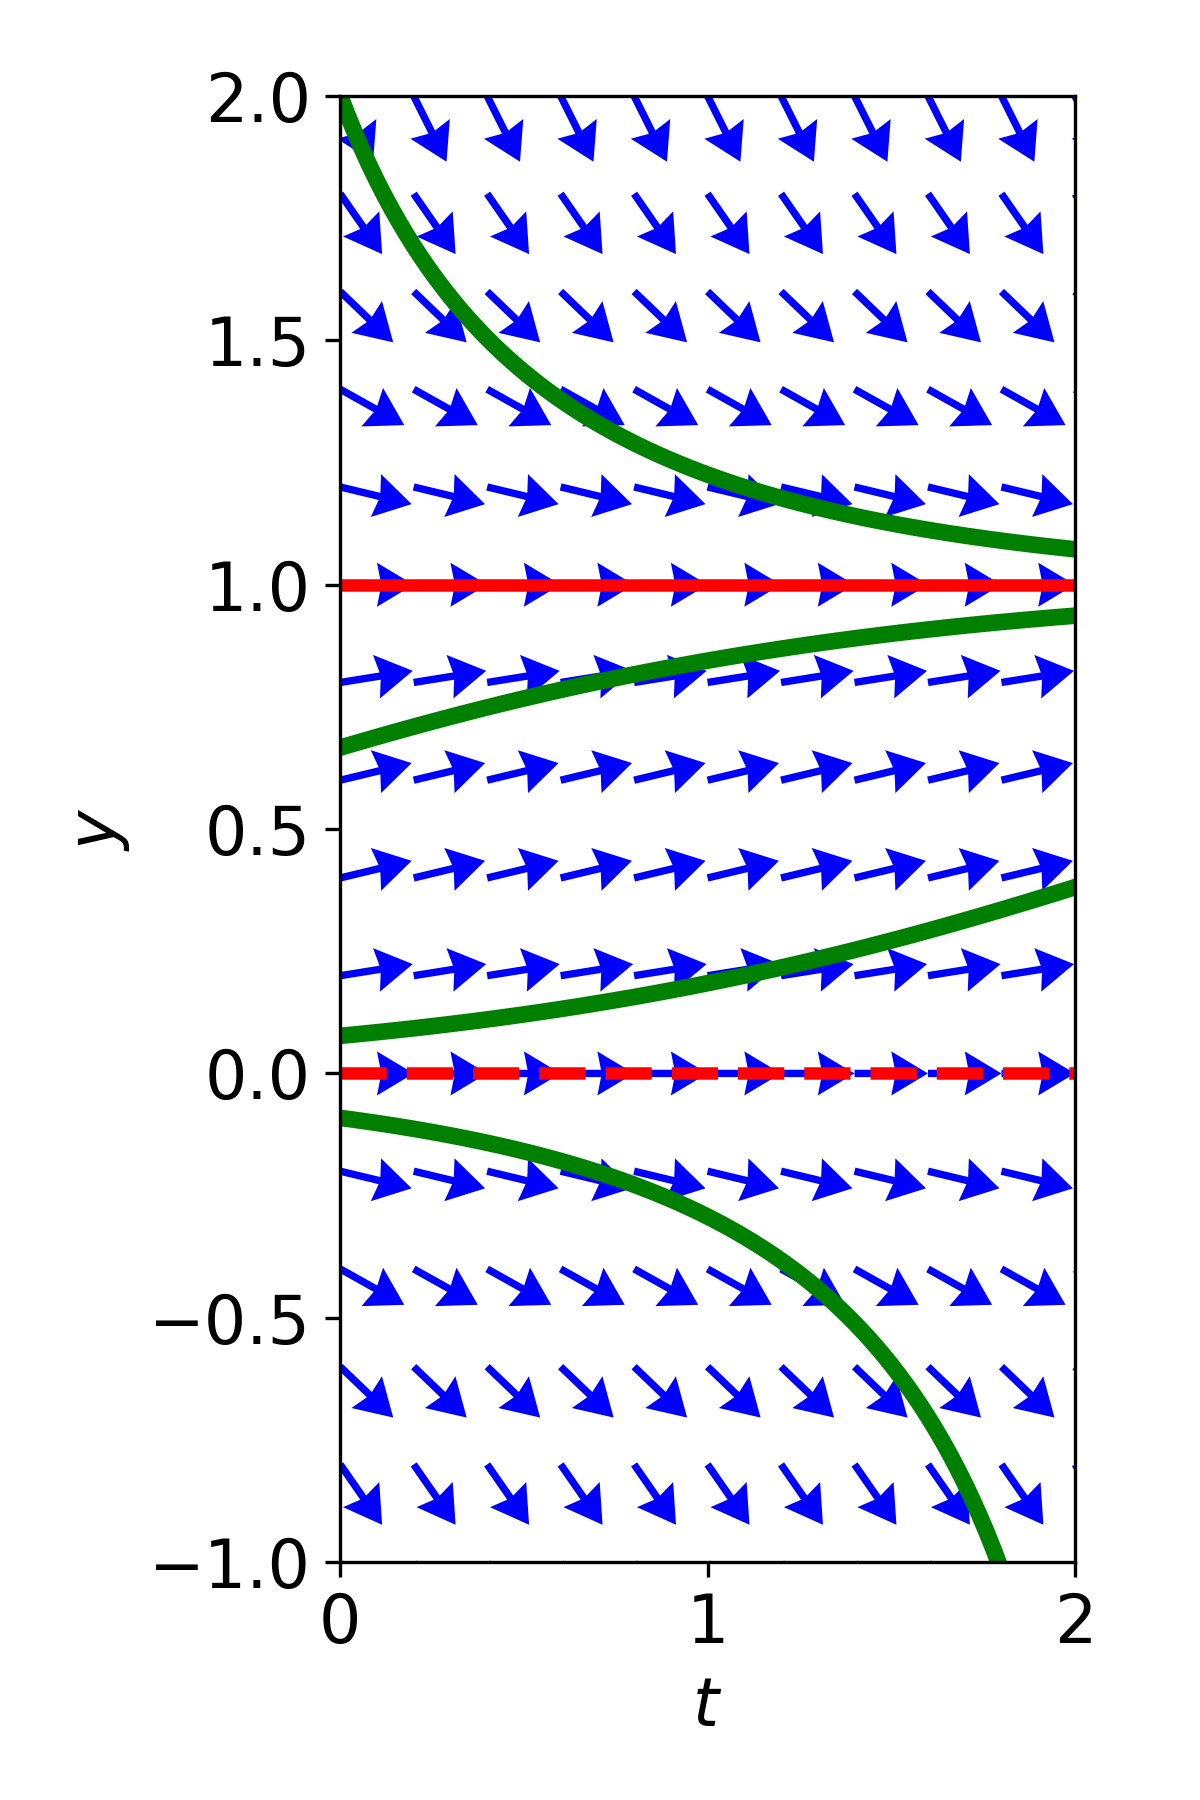
\includegraphics[width=.42\linewidth]{Figures/Section6/logistic_direction_field.png}
\caption{The blue arrows show the direction field for $\der{y}{t}=y(1-y)$. The red lines are stationary solutions and the green curves show example solutions. The dashed and solid lines indicate unstable and stable stationary solutions respectively.}
\label{fig:logistic_direction_field}
\end{figure}

\textbf{Sketching schematic solutions of first-order ODEs}

In order to sketch a first-order ODE given by
\[
\der{y}{x}=f(x,y) \, ,
\]
\begin{enumerate}
\item Plot all the curves where the gradient is 0 (i.e. $f(x,y)=0$).
\item Determine the sign of $f(x,y)$ in each domain bounded by these curves. This gives the direction of $y$ (increasing or decreasing).
\item Sketch these directions with arrows, with $\displaystyle \nearrow$ where $\displaystyle \der{y}{x}>0$, $\rightarrow$ where $\displaystyle \der{y}{x}=0$, and $\searrow$ where $\displaystyle \der{y}{x}<0$.
\item Starting at some initial value of $y$ on the left of the graph, sketch a solution by following the arrows.
\end{enumerate}

% Source slide 27

\goodbreak
\begin{example}[Lecture]
\label{ex:621}

Without solving, sketch some solutions of the ODE
\[
\der{y}{x}=-y\cos x
\]
for $0\leq x\leq \pi $.

\end{example}
\begin{solution}

The stationary points are when $y=\blank{0}$ or $x=\blank{\frac{\pi }{2}}$.

If $y>0$, then $\der{y}{x}\blank{<0}$ for $0<x<\frac{\pi }{2}$ and $ \der{y}{x}\blank{>0}$ for $\frac{\pi }{2}<x<\pi $.

If $y<0$, then $\der{y}{x}\blank{>0}$ for $0<x<\frac{\pi }{2}$ and $ \der{y}{x}\blank{<0}$ for $\frac{\pi }{2}<x<\pi$.

\begin{center}
\ifcsname insertBlanks\endcsname
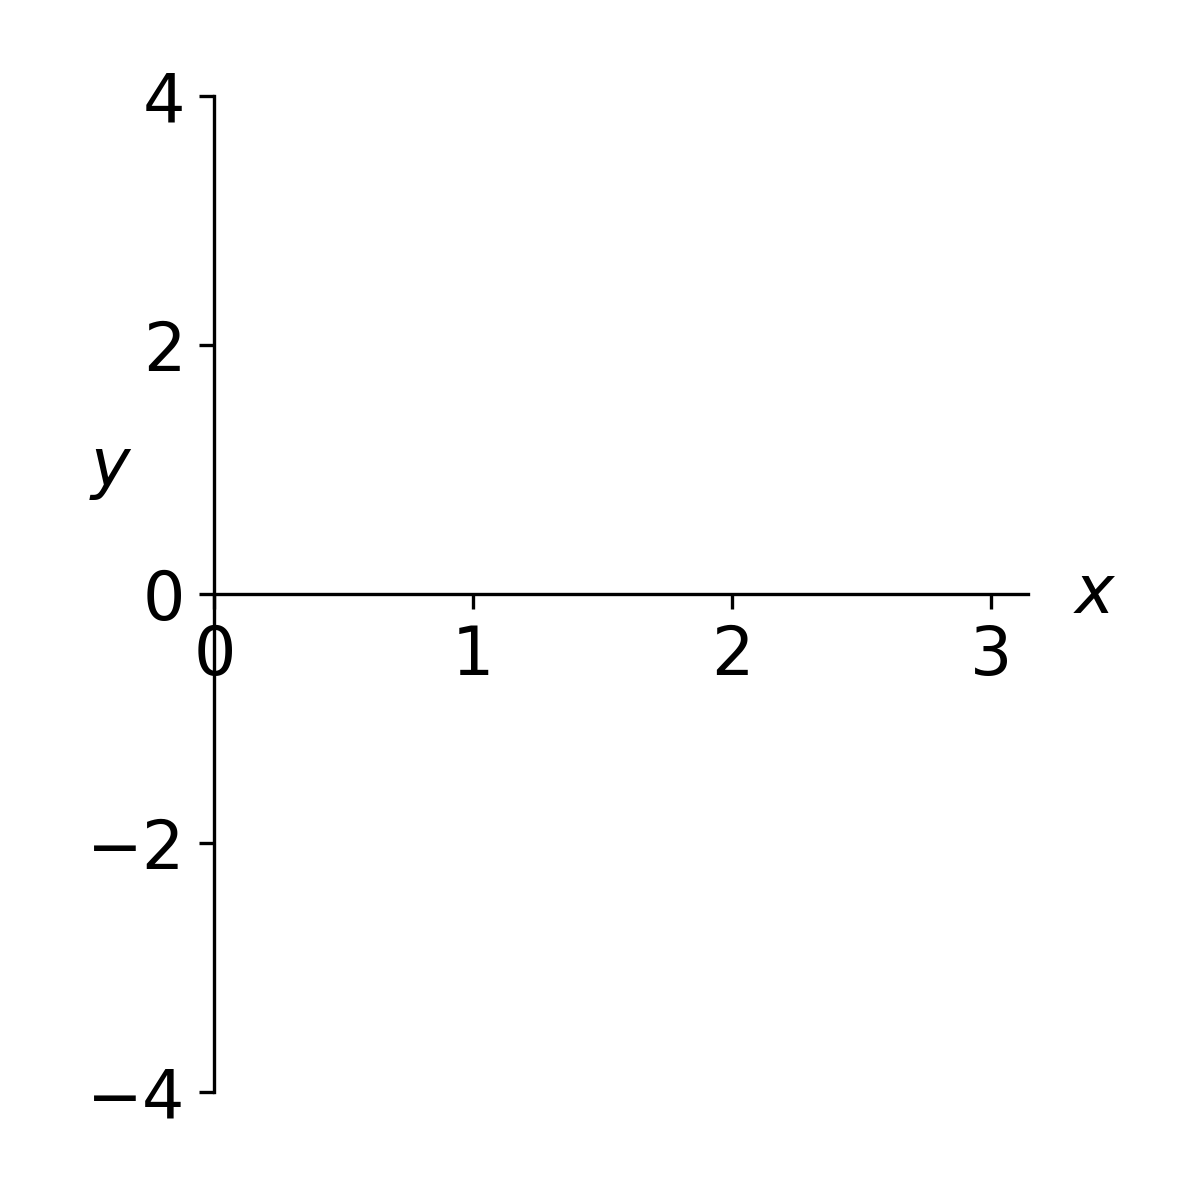
\includegraphics[width=.55\linewidth]{Figures/Section6/example_621_axes.png}
\else
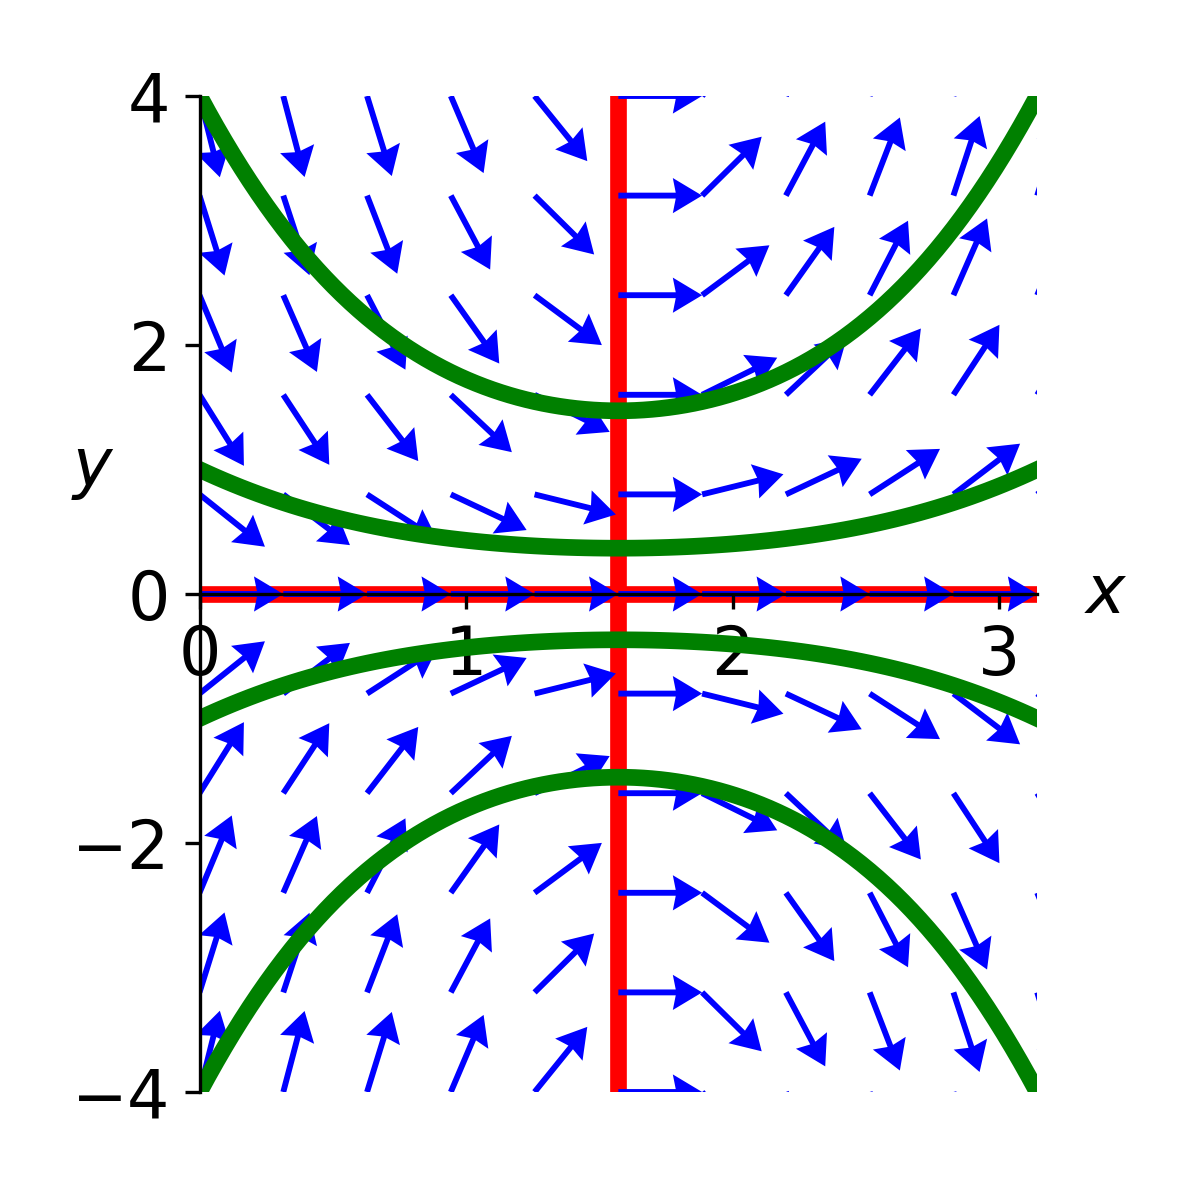
\includegraphics[width=.55\linewidth]{Figures/Section6/example_621_complete.png}
\fi
\end{center}

\end{solution}

% Source slide 29

\textbf{Autonomous ODEs and the stability of stationary solutions}

An autonomous first order ODE is of the form
\[
\der{y}{t}=f(y)
\]
i.e. it does not explicitly depend on $t$. Its stationary solutions, given by $f(y)=0$, depend only on the value of $y$. Therefore, if $y={y}^{\ast }$ and $f\left({y}^{\ast }\right)=0$, then $y={y}^{\ast }$ for all $t$.

% Source slide 30

Consider again the ODE in equation \eqref{eq:logisticODE} 
\[
\der{y}{t}=y(1-y) \, ,
\]
plotted in figure \ref{fig:logistic_direction_field}. The dashed red line at $y=0$ is an unstable stationary solution. If our $y$-value deviates slightly from the line then it continues to get further away. The solid red line at $y=1$ is a stable stationary solution. If our $y$-value deviates slightly from the line, then it gets pulled back towards it.

\goodbreak
\begin{example}[Lecture]
\label{ex:622}

Without solving, sketch solutions of $\der{y}{x}=y(1-y)(1+y)$ for $x\geq 0$ and comment on the stability of the stationary solutions.

\end{example}
\begin{solution}

The stationary solutions are $y=\blank{0,1}$, or $\blank{-1}$. Determine the sign in each region

{\renewcommand{\arraystretch}{1.5}
\begin{center}\begin{tabular}{|c|c|}
\hline
$y<-1$ & $\blank{y'>0}$\\
$-1<y<0$ & $\blank{y'<0}$\\
$0<y<1$ & $\blank{y'>0}$\\
$y>1$ & $\blank{y'<0}$\\
\hline
\end{tabular}\end{center}}

Sketch the solutions
\begin{center}
\ifcsname insertBlanks\endcsname
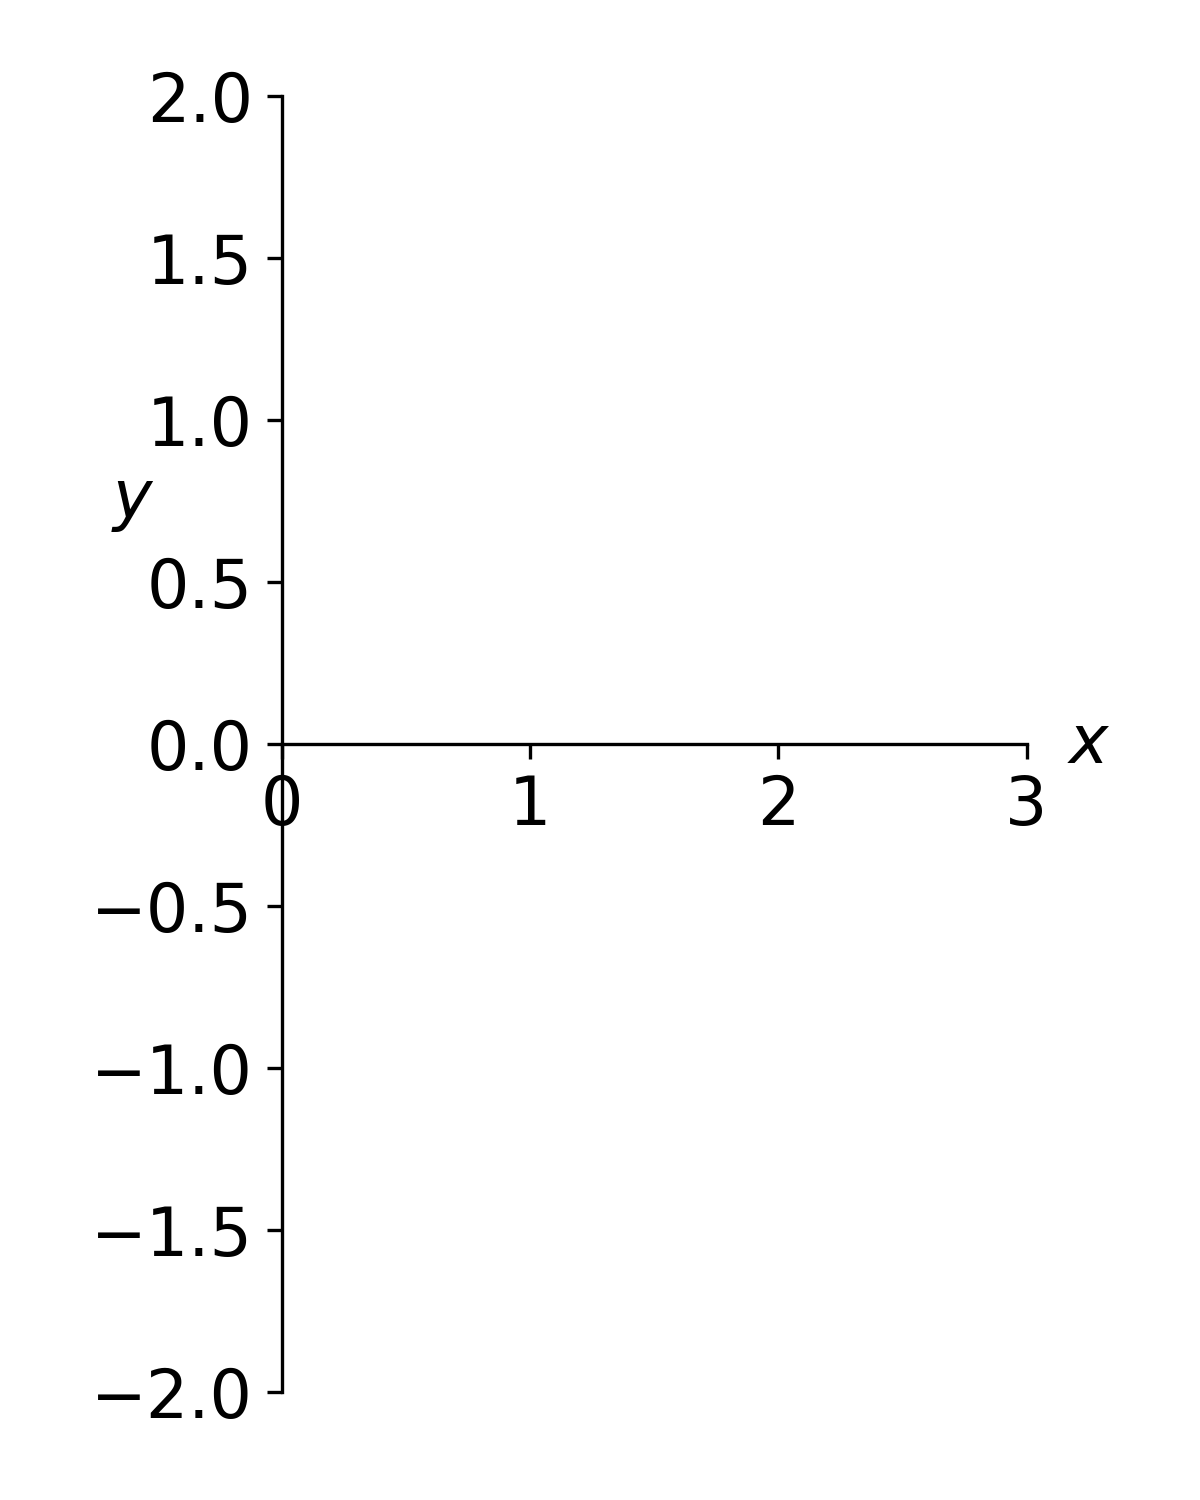
\includegraphics[width=.42\linewidth]{Figures/Section6/example_622_axes.png}
\else
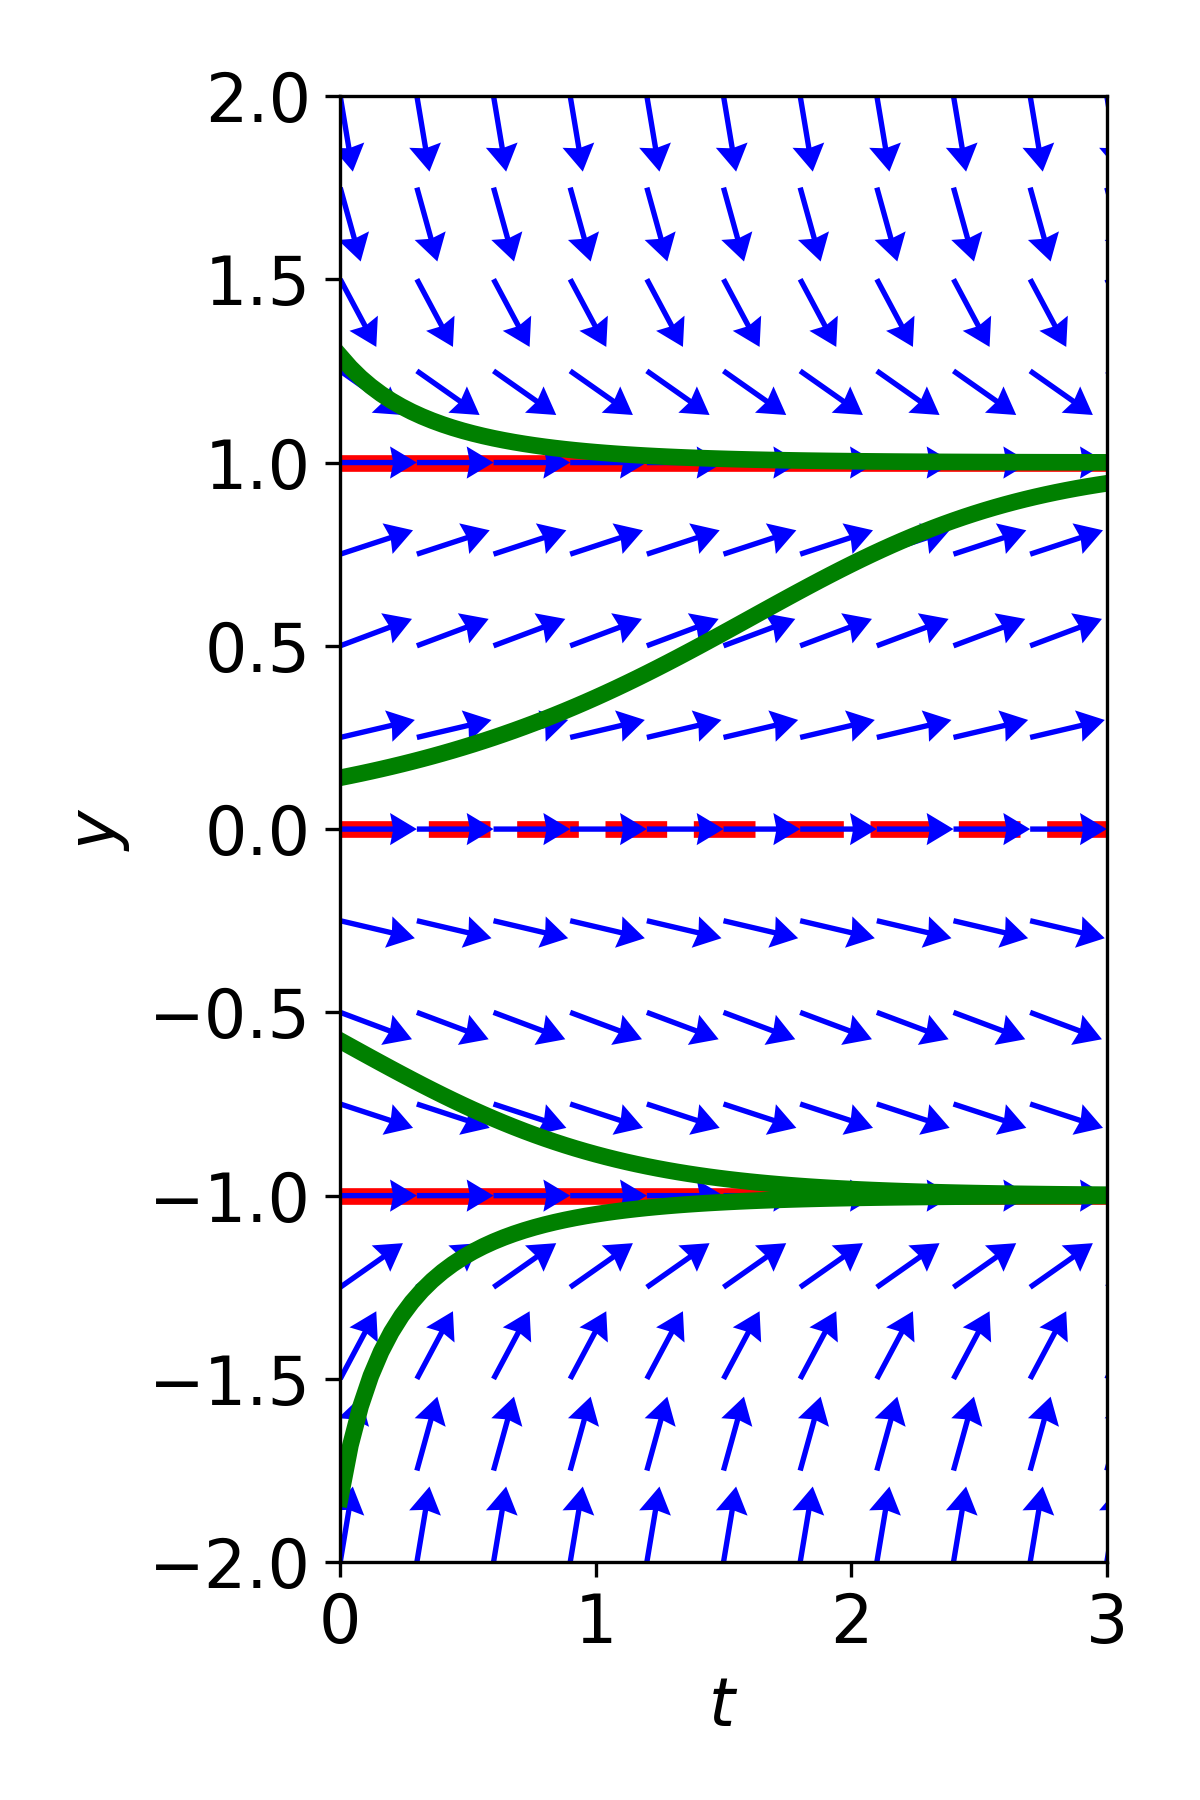
\includegraphics[width=.42\linewidth]{Figures/Section6/example_622_complete.png}
\fi
\end{center}

We can see that the stationary solution $y=\blank{0}$ is unstable, while the solutions $y=\blank{\pm1}$ are stable.

\end{solution}

\begin{recap}{\ref{sec:ode_schematic}}

\item To sketch solutions to a first order ODE without solving;
\begin{enumerate}

\item Identify where ${y}^{\prime }=0$ and draw $\rightarrow$

\item Draw $\uparrow$ where ${y}^{\prime }=+\infty $ and $\downarrow$ where ${y}^{\prime }=-\infty $

\item In between, sketch $\nearrow$ where ${y}^{\prime }>0$ and $\searrow$ where ${y}^{\prime }<0$

\item Sketch solutions by tracing the arrows starting from the left.

\end{enumerate}
\item An autonomous first order ODE is of the form ${y}^{\prime }=f\left(y\right)$

\item These have stationary states $f\left(y\right)=0$.

\item Their stability can be determined from the nearby gradient directions.

\end{recap}

% Source slide 33

\newtexpage
\subsection{Solution of first order ODEs by separation}
\label{sec:ode_separation}

\begin{learningoutcomes}
\item Identify first order ODEs that can be solved by separation and find the general solution
\end{learningoutcomes}

% Source slide 34

An ODE is separable if it can be written in the form
\[
\der{y}{x}=f\left(x\right)g\left(y\right)
\]
We can rearrange to
\[
\frac{1}{g\left(y\right)}\der{y}{x}=f\left(x\right)
\]
noting that the case $g(y)=0$ needs to be considered separately. Integrating both sides with respect to $x$ gives
\[
\int \frac{1}{g\left(y\right)}\der{y}{x}\, {\rm d}x=\int f(x) \, {\rm d}x \, .
\]
From the chain rule, $\displaystyle {\rm d}y=\der{y}{x}\, {\rm d}x$, and therefore
\[
\int \frac{1}{g\left(y\right)}\, {\rm d}y=\int f(x)\, {\rm d}x \, .
\]
This can be integrated (assuming we know how to integrate the functions $f$ and $1/g$). The result is an equation linking $x$ and $y$, including an arbitrary constant, i.e. a general solution.

For example, consider the ODE
\[
\der{y}{x}={x}^{2}{y}^{2}
\]
Note that $y=0$ is a solution. When $y\neq 0$ we can separate the ODE as
\[
\int \frac{1}{{y}^{2}}\, {\rm d}y=\int {x}^{2}\, {\rm d}x \, .
\]
Evaluating the integrals gives
\[
-\frac{1}{y}+{C}_{1}=\frac{1}{3}{x}^{3}+{C}_{2} \, .
\]
For the general solution you can always combine the arbitrary constants of integration, so we will define $C=C_2-C_1$. Then the above can be rearranged to find the general solution
\[
y=-\frac{1}{\frac{1}{3}{x}^{3}+C}
\]
If we are given an initial condition, this allows us to specify $C$ and find the particular solution. For example, given that $y=1$ when $x=0$, we find $C=-1$, and so our particular solution is
\[
{y} = -\frac{1}{\frac{1}{3}{x}^{3}-1}
\]

\goodbreak
\begin{example}[DIY]
\label{ex:631}

Find the general solution of the unimolecular reaction ODE
\[
\der{A}{t}=-kA
\]
\end{example}
\begin{blanksol}

% Source slide 39

Separating the variables gives
\[
\frac{1}{A}\der{A}{t}=-k\, .
\]
Integrating both sides with respect to $t$ gives
\begin{align*}
\int\frac{1}{A}\,dA&=-\int k\, {\rm d}t \, ,\\
\therefore\ln|A|&=-kt+C \, ,\\
|A|&=e^{-kt+C} \, ,\\
\therefore A&=A_0e^{-kt}\, .
\end{align*}
Note this includes the stationary solution $A=0$. A sketch is provided below.
\begin{center}
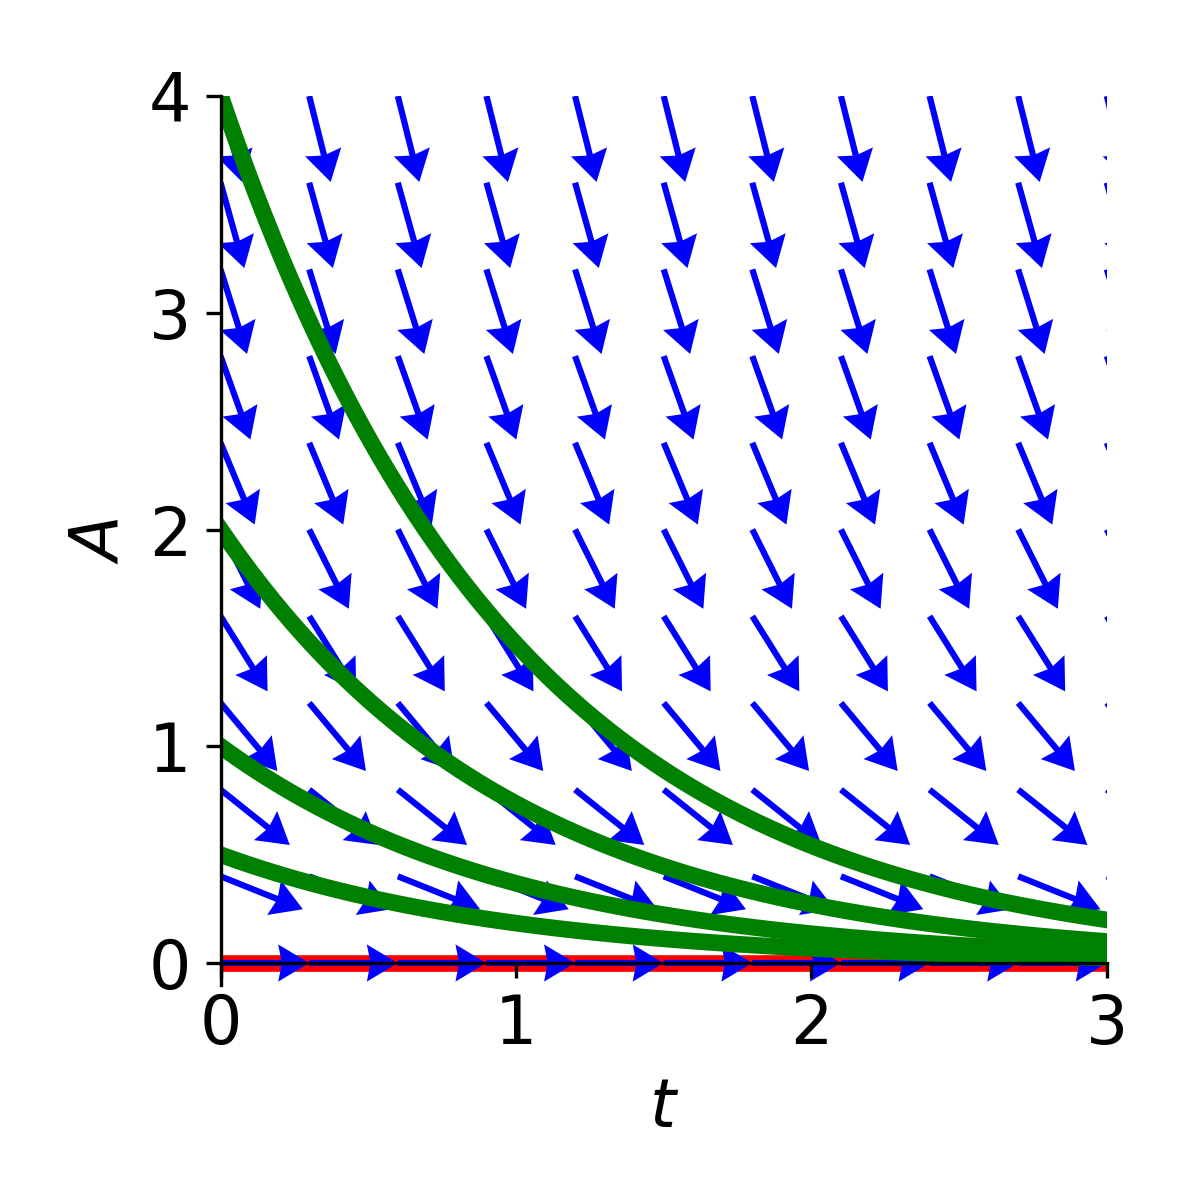
\includegraphics[width=0.4\textwidth, alt={Sketch of solutions to the unimolecular reaction equation.}]{Figures/Section6/sketched_solutions_ex633.png}
\end{center}
\end{blanksol}

% Source slide 40

\goodbreak
\begin{example}[Lecture]
\label{ex:632}

Consider the differential equation
\[
\der{y}{t}=y\left(1-y\right) \quad \text{for} \quad t\geq 0
\]

Find the general solution and also the particular solutions satisfying $y=-0.01, 0.01, 0.5 , 2$ when $t = 0$. Compare with the diagram from section 6.2. What happens when $y=0$ or $1$?

\end{example}
\begin{solution}

% Source slide 41

Separating the variables gives
\[
\blank{\frac{1}{y(1-y)}\der{y}{t}=1}
\]
(assuming $y\neq0$ and $y\neq1$). Using partial fractions on the left hand side gives
\[
\blank{\frac{1}{y(1-y)}=\frac{1}{y}+\frac{1}{1-y}}\, .
\]
Integrating both sides with respect to $t$ gives
\begin{gather*}
\blank{\int\left(\frac{1}{y}+\frac{1}{1-y}\right)\, {\rm d}y=\int \, {\rm d}t}\, ,\\
\therefore\blank{\ln|y|-\ln|1-y|=t+C}\, ,\\
\therefore\blank{\frac{y}{1-y}=Ae^t}\, .
\end{gather*}
Then, $\blank{y(1+Ae^t)=Ae^t}$ so
\[
y=\blank{\frac{Ae^t}{1+Ae^t}}\qquad\text{or}\qquad y=\blank{\frac{1}{Be^{-t}+1}} \, .
\]

% Source slide 42

If $y=\frac{1}{Be^{-t}+1}$, when $t=0$, $y=\blank{\frac{1}{B+1}}$ so $B=\blank{\frac{1}{y}-1}$.
\begin{center}
\renewcommand{\arraystretch}{1.5}
\begin{tabular}{|c|c|c|c|c|}\hline
$y$ & $-0.01$ & $0.01$ & $0.5$ & $2$\\
$B$ & $\blank{-101}$ & $\blank{99}$ & $\blank{1}$ & $\blank{-1/2}$\\\hline
\end{tabular}
\end{center}
So, the four solutions are
\begin{align*}
y_0&=\blank{\frac{1}{1-101e^{-t}}}\, ,&
y_1&=\blank{\frac{1}{1+99e^{-t}}}\, ,\\
y_2&=\blank{\frac{1}{1+e^{-t}}}\, ,&
y_3&=\blank{\frac{1}{1-\frac12e^{-t}}}\, .
\end{align*}

% Source slide 43

For $t\geq0$, we have $0<{e}^{-t}\leq 1$. So, ${y}_{0}\to \blank{-\infty }$ as $t\to \blank{\ln \left(101\right)\approx 4.6}$.

All of ${y}_{1}, {y}_{2},{y}_{3}\to \blank{1}$ as $t\to \infty $. Compare this with the plot in figure \ref{fig:logistic_direction_field}.

We excluded the cases where $y=0$ and $y=1$; these are also particular solutions to the ODE. 
\end{solution}

% Source slide 44

\begin{exammistake}

If $y$ is a solution to an ODE, in general, $y+C$ is not.
\begin{quote}
    \textbf{25/26 Exam Q6(a)(ii).} Find the general solution of the following ODE, assuming $y\neq0$.
    \[
    \der{y}{x}={y}^{2}\cos x
    \]
\end{quote}
By separation, the answer is $-\frac{1}{y}=\sin x+C$ $\therefore y=-\frac{1}{C+\sin x}$.

The common mistake was performing the separation correctly, but then writing the solution with a separate constant e.g. $y=-\frac{1}{\sin x}+\frac{1}{C}$ or $y=-\frac{1}{\sin x}+C$.
\end{exammistake}

% Source slide 45

\begin{recap}{\ref{sec:ode_separation}}

\item An ODE is separable if it can be written in the form
\[
\der{y}{x}=f\left(x\right)g(y)
\]

\item It can be separated into the integral equation
\[
\int \frac{1}{g\left(y\right)}\, {\rm d}y=\int f(x)\, {\rm d}x
\]

\item Evaluating the integrals and combining the integration constants gives the general solution.

\end{recap}

% Source slide 46

\newtexpage
\subsection{Solution of homogeneous first order ODEs}
\label{sec:ode_homogeneous}

\begin{learningoutcomes}
\item Identify homogeneous first order ODEs and find their general solution
\end{learningoutcomes}

% Source slide 47

A homogeneous first-order ODE is one that can be written in the form
\[
\der{y}{x}=f\left(\frac{y}{x}\right)
\]
and can be solved using the substitution $v=y/x$ i.e. $y=vx$. Using the product rule
\[
\der{y}{x}=v\der{x}{x}+x\der{v}{x}=v+x\der{v}{x}
\]

Therefore, the ODE becomes
\[
v+x\der{v}{x}=f\left(v\right) \, ,
\]
which can be solved by separation, as we can see by rearranging as
\[
\left(\frac{1}{f\left(v\right)-v}\right)\der{v}{x}=\frac{1}{x} \, .
\]
Note, if $f\left(v\right)=v$ then the above does not apply and we just have $\der{v}{x}=0$. 

Consider the example
\[
\der{y}{x}=\frac{y}{x}+\frac{{y}^{2}}{{x}^{2}}
\]
Using the substitution $v=y/x$, i.e. $y=vx$, we have $\der{y}{x}=v+x\der{v}{x}$. The equation becomes 
\[
v+x\der{v}{x}=v+{v}^{2} \quad \text{or} \quad x\der{v}{x}={v}^{2}
\]
which separates to
\[
\int \frac{1}{{v}^{2}} {\rm d}v=\int \frac{1}{x}\, {\rm d}x \, .
\]
This integrates to 
\[
-\frac{1}{v}=\ln \left|x\right|+C \quad \text{or} \quad v=-\frac{1}{\ln \left|x\right|+C} \, .
\]
Substituting back in $y=vx$, we find
\[
y=-\frac{x}{\ln \left|x\right|+C}
\]
Note that, again, the constants of integration are combined here. This is the general solution, not accounting for the case when $y=0$, which is also a solution to the equation.

\goodbreak
\begin{example}[Lecture]
\label{ex:641}

Find the general solution of the homogeneous equation
\[
\der{y}{x}=\frac{x+2y}{2x-y}
\]

\end{example}
\begin{solution}

We substitute $y=vx$, so that $y'=v'x+v$. The ODE then becomes
\[
\begin{gathered}
\blank{{v}^{\prime }x+v=\frac{1+2v}{2-v}}
\\[4pt]
\therefore \blank{{v}^{\prime }x=\frac{1+2v-v\left(2-v\right)}{2-v}\equiv \frac{{v}^{2}+1}{2-v}}
\end{gathered}
\]
Separating the variables gives $\blank{\int \frac{2-v}{1+{v}^{2}}\, {\rm d}v=\int \frac{1}{x}\, {\rm d}x}$

% Source slide 51

The integral on the left-hand side is
\begin{align*}
\int\frac{2-v}{1+v^2}\,{\rm d}v
&=\blank{\int\frac{2}{1+v^2}\,{\rm d}v-\int\frac{v}{1+v^2}\,{\rm d}v}\\
&=\blank{2\tan^{-1}v-\frac12\ln(1+v^2)}\, .
\end{align*}
Therefore,
\[
\blank{2\tan^{-1}v-\frac12\ln(1+v^2)=\ln|x|+C}\, .
\]
Taking the exponential of both sides gives
\[
\blank{{\left(1+\frac{{y}^{2}}{{x}^{2}}\right)}^{-\frac{1}{2}}{e}^{2{\tan }^{-1}\left(\frac{y}{x}\right)}} \blank{=Ax}
\]
Rearranging, we can write it as
\[
\blank{{e}^{2{\tan }^{-1}\left(\frac{y}{x}\right)}} \blank{=A\sqrt{{x}^{2}+{y}^{2}} .}
\]
This is a solution in implicit form.
\end{solution}

% Source slide 53

\goodbreak
\begin{example}[Video]
\label{ex:642}

Find the general solution to the following ODE
\[
\der{x}{t}=\frac{x}{t}+3\tan \left(\frac{x}{t}\right)
\]

\end{example}
\begin{solution}

Using the substitution $x=vt$, the ODE becomes $\blank{\der{v}{t}t+v=v+3\tan v}$ or $\blank{\der{v}{t}t=3\tan v}$.

Separating the variables gives $\blank{\int \cot v\, {\rm d}v=3\int \frac{1}{t}\, {\rm d}t}$.

Evaluating the integral on the left-hand side gives
\[
\int \cot v \, {\rm d}v=\blank{\int \frac{\cos v}{\sin v}\, {\rm d}v=\ln |\sin v|+C}
\]
And so,
\[
\blank{\ln |\sin v|=3\ln \left|t\right|-C \therefore \sin v=A{t}^{3}}
\]
which we can leave in implicit form as
\[
\blank{\sin \frac{x}{t}=A{t}^{3}} \, .
\]
\end{solution}

% Source slide 54

\begin{recap}{\ref{sec:ode_homogeneous}}

\item A first order ODE is homogeneous if it can be written in the form
\[
\der{y}{x}=f\left(\frac{y}{x}\right)
\]

\item It may not be obvious that the ODE is homogeneous without rearranging.

\item Homogeneous ODEs can be solved using the substitution $y=vx$ to give a separable ODE since
\[
\der{y}{x}=v+x\der{v}{x}
\]

\end{recap}

\newtexpage
\subsection{Solution of Linear Ordinary Differential Equations}
\label{sec:ode_linear}

\begin{learningoutcomes}
\item Identify linear ODEs and find their general solution using the integrating factor method
\end{learningoutcomes}

% Source slide 56

A linear (first-order) ODE is of the form
\[
\der{y}{x}+P\left(x\right)y=Q(x) \, .
\]
It is a linear expression of the terms $y$ and $\der{y}{x}$. It can be solved using the ``integrating factor''
\[
I(x)={e}^{\int P\left(x\right)\, {\rm d}x} \, .
\]
The first step is to multiply the equation through by $I(x)$
\[
{e}^{\int P\left(x\right)\, {\rm d}x}\der{y}{x}+P\left(x\right){e}^{\int P\left(x\right)\, {\rm d}x}y={e}^{\int P\left(x\right)\, {\rm d}x}Q(x)
\]
Notice that, since $\der{}{x}\int P\left(x\right)\, {\rm d}x=P(x)$, by the chain rule
\[
\der{}{x}\left(y{e}^{\int P\left(x\right)\, {\rm d}x}\right)={e}^{\int P\left(x\right)\, {\rm d}x}\der{y}{x}+P\left(x\right){e}^{\int P\left(x\right)\, {\rm d}x}y
\]
Therefore, the equation can be re-written as
\[
\der{}{x}\left(yI(x)\right)=Q\left(x\right)I(x) \, .
\]
And so, integrating both sides with respect to $x$ gives
\[
yI(x)=\int Q(x)I(x)\,\, {\rm d}x\qquad\text{or}\qquad y=\frac{1}{I(x)}\int Q(x)I(x)\,\, {\rm d}x\, .
\]

% Source slide 58

For example, consider
\[
\der{y}{x}+y\sin x=-2\sin x
\]
The function $P\left(x\right)=\sin x$ so the integrating factor is
\[
I={e}^{\int \sin x\, {\rm d}x}={e}^{-\cos x} \, .
\]
Note that we do not need to write the constant of integration, as it will drop out. Multiplying through by $I$ and using the chain rule
\[
\der{}{x}\left(y{ e}^{-\cos x}\right)=-2{e}^{-\cos x}\sin x \, .
\]

Integrating $\der{}{x}\left(y{ e}^{-\cos x}\right)=-2{e}^{-\cos x}\sin x$ gives
\[
y{ e}^{-\cos x}=-2\int {e}^{-\cos x}\sin x\, {\rm d}x
\]

The right-hand side can be integrated using the substitution $u=-\cos x$
\[
-2\int {e}^{-\cos x}\sin x\, {\rm d}x=-2\int {e}^{u}du=-2{e}^{u}+C
\]

Substituting this back in gives
\[
y{ e}^{-\cos x}=-2{e}^{-\cos x}+C
\]
and so, the general solution to the ODE is
\[
y=-2+C{e}^{\cos x}
\]

% Source slide 60

\goodbreak
\begin{example}[Lecture]
\label{ex:651}

The relative amount of neptunium at any time in the two-step radioactive decay process of uranium can be described by
\[
\der{n}{t}+{\lambda }_{1}n={\lambda }_{2}{e}^{-{\lambda }_{2}t}
\]
where ${\lambda }_{1}$ and ${\lambda }_{2}$ are constant decay rates. Find the general solution for $n$.
\end{example}
\begin{solution}

The integrating factor is
\[
I=\blank{{e}^{\int {\lambda }_{1} \, {\rm d}t}={e}^{{\lambda }_{1}t}}
\]
and so, multiplying through by $I$ the equation can be written as
\[
\blank{\der{}{t}\left({e}^{{\lambda }_{1}t}n\right)={\lambda }_{2}{e}^{\left({\lambda }_{1}-{\lambda }_{2}\right)t}}
\]
Integrating both sides with respect to $t$ gives
\[
\blank{{e}^{{\lambda }_{1}t}n=\int {\lambda }_{2}{e}^{\left({\lambda }_{1}-{\lambda }_{2}\right)t} \, {\rm d}t}
\]
if ${\lambda }_{1}\neq {\lambda }_{2}$:
\[
n=\blank{{e}^{-{\lambda }_{1}t}\left[\frac{{\lambda }_{2}}{{\lambda }_{1}-{\lambda }_{2}}{e}^{\left({\lambda }_{1}-{\lambda }_{2}\right)t}+C\right]=\frac{{\lambda }_{2}}{{\lambda }_{1}-{\lambda }_{2}}{e}^{-{\lambda }_{2}t}+C{e}^{-{\lambda }_{1}t}}
\]
if ${\lambda }_{1}={\lambda }_{2}$:
\[
n=\blank{{e}^{-{\lambda }_{1}t}\left({\lambda }_{2}t+C\right)={\lambda }_{2}t{e}^{-{\lambda }_{1}t}+C{e}^{-{\lambda }_{1}t}}
\]
Note the placement of the constant.

\end{solution}

% Source slide 62

Sometimes it is necessary to rearrange the equation to identify the integrating factor. A common case occurs when the coefficient of the derivative is not 1, e.g. the equation
\[
a(x)\der{y}{x}+b\left(x\right)y=c(x)
\]

Dividing through by $a(x)$ gives the appropriate form
\[
\der{y}{x}+\frac{b\left(x\right)}{a\left(x\right)}y=\frac{c\left(x\right)}{a\left(x\right)}
\]
where $P(x)$ is now $\frac{b\left(x\right)}{a\left(x\right)}$ and $Q(x)$ is now $\frac{c\left(x\right)}{a\left(x\right)}$.

% Source slide 63

\goodbreak
\begin{example}[Video]
\label{ex:652}

Use the integrating factor method to solve the equation
\[
t\der{z}{t}-3z=2{t}^{2}
\]
subject to $z=1$ when $t=1$.

\end{example}
\begin{solution}

Divide through by $t$:
\[
\blank{\der{z}{t}-\frac{3z}{t}=2t}
\]

The integrating factor is
\[
IF=\blank{{e}^{-\int 3/t \, {\rm d}t}={e}^{-3\ln t}={t}^{-3}}
\]

% Source slide 64

Multiplying through by $IF=t^{-3}$ gives
\[
\blank{\der{}{t}\left({t}^{-3}z\right)=2{t}^{-2}}
\]

Integrating both sides gives
\[
z=\blank{{t}^{3}\left({-2t}^{-1}+C\right)=C{t}^{3}-2{t}^{2}}
\]

Given $z=1$ when $t=1$, $z=3\blank{{t}^{3}-2{t}^{2}}$.

\end{solution}

\textbf{Identify that ODE!}

Determine whether the following ODEs are separable, homogeneous and/or linear.

The equation
\[
\frac1x\der{x}{t}+4e^{2t}=0
\]
is \blank{separable and linear}. \par 

The equation
\[
y^2\der{y}{x}+4xy=2x^2
\]
is \blank{homogeneous}.\par 

The equation
\[
\der{y}{x}=x^2+y^2
\]
is \blank{none of the three}.

\goodbreak
\begin{example}[Lecture]
\label{ex:653}
Consider the differential equation
\[
\der{y}{x}=\frac{y}{x}\, .
\]
Find the general solution using
\begin{enumerate}[label=(\alph*)]
\item separation,
\item substitution $y=vx$,
\item the integrating factor.
\end{enumerate}
\end{example}
\begin{solution}
\begin{enumerate}[label=(\alph*)]
\item By separation, we obtain
\[
\blank{\int\frac1y\, {\rm d}y=\int\frac1x\, {\rm d}x} \, .
\]
Integrating gives $\blank{\ln |y|=\ln|x|+C}$, taking the exponential of both sides gives $|y|=\blank{e^{\ln|x|+C}}$ and so 
\[
y=\blank{Ax}  \,.
\]
\item By substitution of $v=y/x$, we obtain
\[
\blank{v'x+v=v}\qquad\therefore\blank{v'x=0}\qquad\text{so}\qquad\blank{v'=0}.
\]
Integrating gives $\blank{v=A}$, therefore 
\[
y=\blank{Ax} \,.
\]
\item Using the integrating factor method, comparing with
\[
\der{y}{x}+P(x)y=Q(x)\, ,
\]
we have $P(x)=\blank{-\frac1x}$ and $Q(x)=\blank{0}$. The integrating factor is
\[
I=\blank{e^{-\int x^{-1} \, {\rm d}x}=e^{-\ln|x|}=|x|^{-1}}\, .
\]
Taking $x>0$ and multiplying through by the IF gives
\[
\blank{\frac1x\der{y}{x}-\frac{y}{x^2}=0}\qquad\text{or}\qquad\blank{\der{}{x}\left(\frac yx\right)=0}\, .
\]
Integrating gives $\blank{\frac yx=A}$, so 
\[
y=\blank{Ax} \,.
\]
Note, this solution also works for $x<0$.
\end{enumerate}
\end{solution}

% Source slide 69

\begin{recap}{\ref{sec:ode_linear}}

\item A first-order linear ODE can be written in the form
\[
\der{y}{x}+P\left(x\right)y=Q(x)
\]

\item Multiplying through by the integrating factor $I(x)={e}^{\int P\left(x\right)\, {\rm d}x}$ allows it to be re-written as
\[
\der{}{x}\left(yI(x)\right)=Q\left(x\right)I(x)
\]
which in many cases can be integrated to find the general solution.

\end{recap}


% Source slide 70

\newtexpage
\subsection{Introduction to second order ODEs}
\label{sec:ode_second}

\begin{learningoutcomes}
\item Recognise a linear second order ODE with constant coefficients.
\item Solve homogeneous ODEs of this form using the auxiliary equation
\item Identify the particular integral and use this to solve inhomogeneous ODEs of this form
\end{learningoutcomes}

% Source slide 71

\textbf{Second Order Ordinary Differential Equations.}

A second-order ODE is an equation of the form
\[
f\left(x,y,\der{y}{x},\der{^2y}{x^2}\right)=0
\]
An example application is modelling mechanical oscillations, such as those shown in Figure~\ref{fig:ode_mechanics}.

\begin{figure}[!htb]
\centering
\subfig{0.4}{Figures/Section6/pendulum.png}{A simple pendulum.}
\subfig{0.4}{Figures/Section6/spring.png}{A mass attached to a spring.}
\caption{Two mechanical systems whose motion can be modelled using second-order differential equations.}
\label{fig:ode_mechanics}
\end{figure}

% Source slide 72

\textbf{Linear 2nd order ODE with constant coefficients}

We will consider 2nd order ODEs that can be written in the form
\[
a\der{^2y}{x^2}+b\der{y}{x}+cy=f(x)
\]
where $a$, $b$, and $c$ are constants. In the case of a mass on a spring, the equation of motion is
\[
m\der{^2x}{t^2}+c\der{x}{t}+kx=f(t) \, ,
\]
where $m$ is the mass, $c$ is the damping/friction coefficient, $k$ is the spring stiffness, and $f(t)$ is the external forcing.

% Source slide 73

\textbf{Homogeneous case}

Take the special case when the right-hand side is zero
\[
a\der{^2y}{x^2}+b\der{y}{x}+cy=0
\]
This is known as the homogeneous case. This should not be confused with homogeneous first-order ODEs in Section~\ref{sec:ode_homogeneous}. For particular values of $m$
\[
y={e}^{mx}
\]
is a solution of this ODE. If $y={e}^{mx}$, then $\der{y}{x}=m{e}^{mx}$ and $\der{^2y}{x^2}={m}^{2}{e}^{mx}$. The equation
\[
a\der{^2y}{x^2}+b\der{y}{x}+cy=0
\]
becomes
\[
{e}^{mx}\left(a{m}^{2}+bm+c\right)=0
\]
This is only satisfied if $m$ is a solution to the quadratic
\[
a{m}^{2}+bm+c=0 \, .
\]
This is known as the \textbf{auxiliary equation}.

\goodbreak
\begin{example}[DIY]
\label{ex:661}

Find the auxiliary equation, and the values of $m$ that satisfy it, for the following ODE
\[
\der{^2y}{x^2}+\der{y}{x}-6y=0 \, .
\]

\end{example}
\begin{blanksol}

% Source slide 76
The auxiliary equation is $ {m}^{2}+m-6=0$
\[
(m+3)(m-2)=0
\]
therefore $m=-3$ and $m=2$.
\vspace{8mm}
\end{blanksol}

\textbf{General solution of 2nd order homogeneous linear ODEs with constant coefficients}

In general, the auxiliary equation has two solutions, ${m}_{1}$ and ${m}_{2}$. Therefore, ${y}_{1}={e}^{{m}_{1}x}$ and ${y}_{2}={e}^{{m}_{2}x}$ are both solutions of the ODE. If the roots are real and distinct (${m}_{1}\neq {m}_{2}$), the general solution is
\[
y=A{y}_{1}+B{y}_{2}=A{e}^{{m}_{1}x}+B{e}^{{m}_{2}x} \, ,
\]
where $A$ and $B$ are arbitrary constants. If the roots are real and repeated (${m}_{1}={m}_{2}=m$), the general solution is
\[
y=A{e}^{mx}+B{xe}^{mx} \, .
\]
For second-order ODEs, the general solution always has two arbitrary constants.

As there are two arbitrary constants, finding the particular solution requires two additional bits of information, for example:
\begin{itemize}
\item Boundary conditions: the value of $y$ at two different $x$ values, e.g. $y(x_1)$ and $y(x_2)$.
\item Initial conditions: the value of $y$ and $y'$ at one $x$ value, e.g. $y(x_1)$ and $y'(x_1)$.
\end{itemize}

% Source slide 79

\goodbreak
\begin{example}[Lecture]
\label{ex:662}
Find the solution of the following ODE
\[
\der{^2y}{x^2}-4\der{y}{x}+4y=0
\]
given $y(0)=0$ and $y'(0)=1$\, .
\end{example}
\begin{solution}
The auxiliary equation is
\[
\blank{m^2-4m+4=0}\qquad\therefore\blank{(m-2)^2=0}\, ,
\]
and so
\begin{align*}
y&=\blank{Ae^{2x}+Bxe^{2x}}\, ,\\
\therefore y'&=\blank{2Ae^{2x}+2Bxe^{2x}+Be^{2x}}\, .
\end{align*}
When $x=0$, $y=\blank{A}$, so $A=\blank{0}$. When $x=0$, $y'=\blank{B}$, so $B=\blank{1}$. So, the particular solution is
\[
y=\blank{xe^{2x}} \, .
\]
\end{solution}

% Source slide 80
\goodbreak
\begin{example}[Video]
\label{ex:663}
Consider a reversible chemical reaction $A\rightleftharpoons B$, where $A\to B$ with rate $k_1$ and $B\to A$ with rate $k_2$. Also, $B$ is equally likely to decay to a third species with rate $k_2$. This can be described by the first order ODEs
\[
\der{A}{t}=-k_1A+k_2B\qquad
\der{B}{t}=-2k_2B+k_1A.
\]
Combine these into a single second order ODE for $B$ and find the general solution when $k_1=3$ and $k_2=2$ (in suitable units).
\end{example}
\begin{solution}
Differentiating the ODE for $B$ gives
\[
\der{^2B}{t^2}=\blank{-2k_2\der{B}{t}+k_1\der{A}{t}}\, .
\]
Substituting the ODE for $A$ into this gives
\[
\der{^2B}{t^2}=\blank{-2k_2\der{B}{t}+k_1(-k_1A+k_2B)}\, .
\]
Then from the ODE for $B$ we have $k_1A=\blank{\der{B}{t}+2k_2B}$. Substituting this in gives
\[
\der{^2B}{t^2}=\blank{-2k_2\der{B}{t}-k_1\left(\der{B}{t}+k_2B\right)}\, ,
\]
which can be rearranged as
\[
\blank{\der{^2B}{t^2}+(k_1+2k_2)\der{B}{t}+k_1k_2B}=0.
\]
If $k_1=3$ and $k_2=2$, this becomes
\[
\blank{\der{^2B}{t^2}+7\der{B}{t}+6B}=0\, .
\]
The auxiliary equation is
\[
\blank{m^2+7m+6=0}\qquad\text{or}\qquad\blank{(m+6)(m+1)=0}\, .
\]
So, the general solution for $B$ is
\[
B=\blank{\alpha e^{-6t}+\beta e^{-t}}\, .
\]
\end{solution}

% Source slide 81

\textbf{Complex solutions to the auxiliary equation.}

Recall the auxiliary equation
\[
a{m}^{2}+bm+c=0\, ,
\]
if its roots, ${m}_{1}$ and ${m}_{2}$, are complex and $a$, $b$, and $c$ are real (this is the only case we will consider here) then ${m}_{1}$ and ${m}_{2}$ are conjugates of one another, so ${m}_{1}=m+ik$ and ${m}_{2}=m-ik$ and so, the general solution is given by
\[
y=W{e}^{(m+ik)x}+Z{e}^{(m-ik)x} ={e}^{mx}\left(W{e}^{ikx}+Z{e}^{-ikx}\right) \, .
\]
Using Euler's formula gives ${e}^{ikx}=\cos (kx)+i\sin \left(kx\right)$ and ${e}^{-ikx}=\cos (kx)-i\sin \left(kx\right)$. So, $y={e}^{mx}\left[\left(W+Z\right)\cos \left(kx\right)+i\left(W-Z\right)\sin \left(kx\right)\right]$. Since the solution should be real, $A=W+Z$ and $B=i\left(W-Z\right)$ should be real, which implies $Z=\frac{1}{2}(A+iB)$ and $W=\frac{1}{2}\left(A-iB\right)=\overline{Z}$.

So, if the solutions to the auxiliary equation are ${m}_{1}=m+ik$ and ${m}_{2}=m-ik$ then the general solution is
\begin{align}
y={e}^{mx}\left[A\cos \left(kx\right)+B\sin \left(kx\right)\right]
\end{align}
which can also be written as
\[
y=\overline{Z}{e}^{(m+ik)x}+Z{e}^{(m-ik)x} \, ,
\]
where $Z=\frac{A+iB}{2}$.

% Source slide 84

\goodbreak
\begin{example}[Lecture]
\label{ex:664}
Find the general solution to the following differential equations.
\begin{enumerate}[label=(\alph*)]
\item $\displaystyle \der{^2x}{t^2}=-3x$
\item $\displaystyle \der{^2y}{x^2}-2\der{y}{x}+3y=0$
\end{enumerate}
\end{example}
\begin{solution}
\begin{enumerate}[label=(\alph*)]
\item The auxiliary equation is
\[
\blank{m^2=-3}\qquad\therefore m=\pm\blank{\sqrt3 i}\, ,
\]
and so $x=\blank{A\cos(\sqrt3 t)+B\sin(\sqrt3 t)}$.

\item The auxiliary equation is
\[
\blank{m^2-2m+3}=0\, ,
\]
\[
\therefore m=\blank{1 \pm \frac{\sqrt{4-12}}2=1\pm\sqrt2 i}\, .
\]
Therefore $y=\blank{e^x\left[A\cos(\sqrt2 x)+B\sin(\sqrt2 x)\right]}$.
\end{enumerate}
\end{solution}

% Source slide 86

\textbf{Behaviour of solutions}

If the roots of the auxiliary equation, $m_1$ and $m_2$, are real, in general solutions will either
\begin{itemize}
\item decay to zero if $m_1<0$ and $m_2<0$, e.g. $y=e^{-x}+e^{-2x}$;
\item tend to a constant if $m_1<0$ and $m_2=0$, e.g. $y=1+e^{-2x}$; or
\item grow indefinitely if $m_1>0$ or if $m_2>0$ or $m_1,m_2=0$, e.g. $y=e^x+e^{-2x}$ or $y=1+\frac{x}{2}$.
\end{itemize}
See figure \ref{fig:ode_behaviour}(a). 

Otherwise, if the roots of the auxiliary equation, ${m}_{1}$ and ${m}_{2}$, are 
\begin{itemize} 
\item imaginary, then the solutions will oscillate e.g. $y=\cos \left(2x\right)$
\item complex, then the solutions oscillate with angular frequency given by the imaginary part and decay/grow based on the sign of the real part e.g. $y={2e}^{-x}\cos \left(2x\right)$ (decaying) and $y={\frac{1}{2}e}^{x/4}\cos \left(2x\right)$ (growing).
\end{itemize}
See figure \ref{fig:ode_behaviour}(b). 

\begin{figure}[!htb]
\centering
\subfig{0.47}{Figures/Section6/real_root_behaviour.png}{Real auxiliary roots.}
\subfig{0.47}{Figures/Section6/complex_root_behaviour.png}{Imaginary and complex auxiliary roots.}
\caption{Examples of the behaviour of solutions to homogeneous linear second-order ODEs with constant coefficients. The signs of the real parts determine growth or decay; non-zero imaginary parts produce oscillations.}
\label{fig:ode_behaviour}
\end{figure}

% Source slide 88

\textbf{Worked example: a simple pendulum.}

A pendulum with length 1 m and mass 1 kg has angle $\theta $ with the vertical axis, which changes with time $t$ according to the differential equation
\[
\der{^2\theta}{t^2}+2\lambda \der{\theta}{t}+g\theta =0 \, ,
\]
where $g\approx9.81\,\mathrm{m}\,\mathrm{s}^{-2}$ is the acceleration due to gravity and $\lambda >0$ is a damping/friction parameter. How does changing $\lambda $ affect the solution?

\vspace{4mm}
\begin{center}
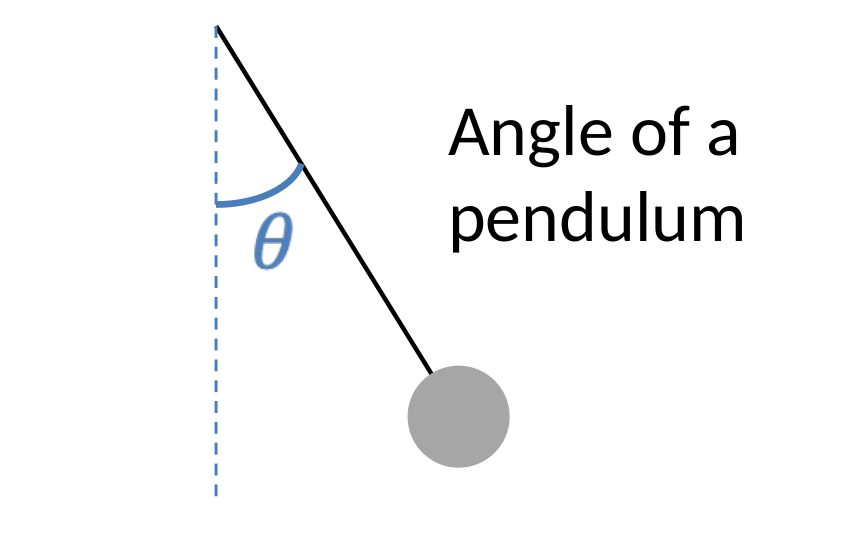
\includegraphics[width=.45\linewidth, alt={Sketch of a simple pendulum with angle $\theta$ to the vertical axis.}]{Figures/Section6/pendulum.png}
\end{center}
\vspace{4mm}

The roots of the auxiliary equation are ${m}_{+}=-\lambda +\sqrt{{\lambda }^{2}-g} $ and ${m}_{-}=-\lambda -\sqrt{{\lambda }^{2}-g} $.

\begin{itemize}
\item \textbf{No damping} ($\lambda =0$): The auxiliary roots are imaginary
\[
{m}_{+}=\sqrt{g}i \quad \text{and} \quad {m}_{-}=-\sqrt{g}i \, .
\]
The solution is $\theta=A\cos(\sqrt{g}t)+B\sin(\sqrt{g}t)$, so the pendulum keeps oscillating forever.

\item \textbf{Underdamped} ($\lambda <\sqrt{g}$): The auxiliary roots are complex
\[
{m}_{+}=-\lambda +i\sqrt{g-{\lambda }^{2}} \quad \text{and} \quad  {m}_{-}=-\lambda -i\sqrt{g-{\lambda }^{2}} \, .
\]
The general solution is
\[
\theta ={e}^{-\lambda t}\left(A\cos kt+B\sin kt\right)
\]
where $k=\sqrt{g-{\lambda }^{2}}$. So, oscillations decay with time.

\item \textbf{Critical / overdamped} ($\lambda \geq \sqrt{g}$): The auxiliary roots are real
\[
{m}_{+}=-\lambda +\sqrt{{\lambda }^{2}-g} \quad \text{and} \quad {m}_{-}=-\lambda -\sqrt{{\lambda }^{2}-g} \, .
\]
The general solution is $\theta =A{e}^{{m}_{+}t}+B{e}^{{m}_{-}t}$ or $\theta =A{e}^{mt}+B{te}^{mt}$ if ${m}_{+}={m}_{-}=m$. Note that ${m}_{-}\leq {m}_{+}<0$ because $\sqrt{{\lambda }^{2}-g}<\lambda $. So, the solution decays to zero without oscillating.
\end{itemize}
These different regimes can be visualised in the animation in figure \ref{anim:ode_pendulum}.

\begin{figure}
    \iflatexml    
        \bmlRawHTML{<div id="damped-oscillator-widget"></div>} 
        \caption{Interactive plot and visualisation of the solutions to the damped pendulum. Use the slider to change the value of $\lambda$.}
    \else
        \centering
        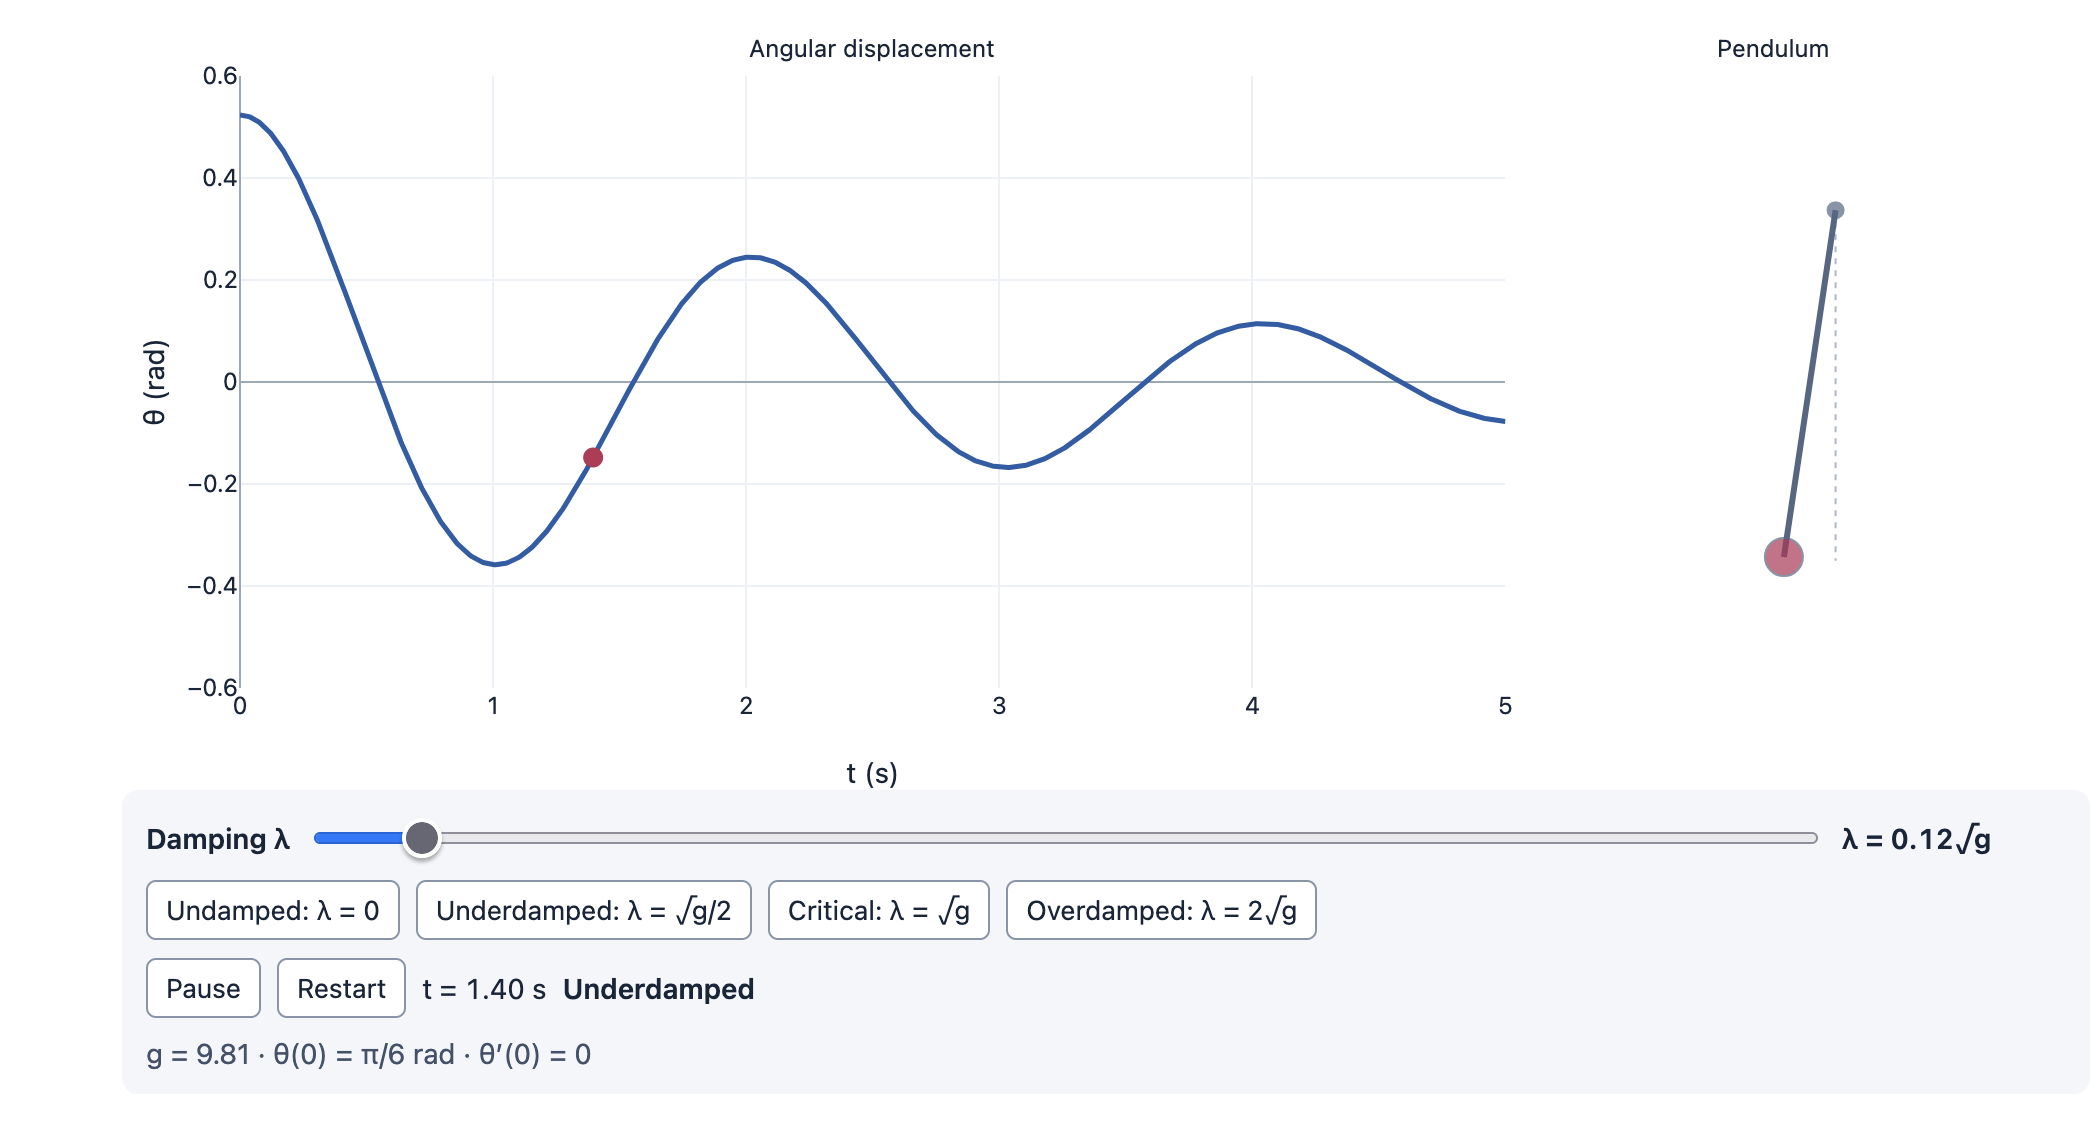
\includegraphics[width=0.8\textwidth]{Figures/Section6/ode_pendulum.png}
        \caption{Screenshot of the interactive plot and visualisation of the solutions to the damped pendulum, available in the HTML version of these notes and \href{https://carlwhitfield.github.io/animations/ode/ode_widget.html}{here}.}
    \fi
    \label{anim:ode_pendulum}
\end{figure}

\newtexpage
\textbf{Inhomogeneous case}

Consider the inhomogeneous second-order ODE
\[
\der{^2y}{x^2}+2\der{y}{x}+y=3x .
\]
A solution is $y=3x-6$ (check by substituting it in). The ``homogeneous part'' is $\der{^2y}{x^2}+2\der{y}{x}+y=0$, which has solution
\[
y=A{e}^{-x}+Bx{e}^{-x} \, .
\]
Therefore
\[
y=3x-6+A{e}^{-x}+Bx{e}^{-x}
\]
also solves the ODE, since the homogeneous part of the solution does not change the left-hand side. This is the general solution to the ODE.

More generally, the solution to
\begin{align}
\label{eq:inhom} a\der{^2y}{x^2}+b\der{y}{x}+cy=f(x)
\end{align}
can be given as
\[
y={y}_{p}+{y}_{h} \, ,
\]
where $y_p$ is a particular integral and $y_h$ is the homogeneous solution.

\textbf{Finding the particular integral}

To find the particular integral, we need to try a solution with a matching form and substitute it in. Examples are given in table \ref{tab:particular_integrals}.

\renewcommand{\arraystretch}{2.0}
\begin{table}[ht]
    \centering
    \begin{tabular}{|p{.25\linewidth}|p{.20\linewidth}|p{.50\linewidth}|}
    \hline
    Type & Example $f(x)$ & Try ${y}_{p}=$\\ \hline
    Polynomial degree $n$ & ${x}^{2}+1$ & $a{x}^{2}+bx+c$\\
    Sine or cosine & $\cos (3x)$ & $a\sin \left(3x\right)+b\cos \left(3x\right)$\\
    Exponential & ${e}^{-x}$ & $a{e}^{-x}$\\
    Product of degree $n$ polynomial and exponential or sine & $\left(x-1\right){e}^{4x}$ \par or \par ${x}^{2}\sin (2x)$ & $\left(ax+b\right){e}^{4x}$ \par or \par $(ax^2+bx+c)\sin(2x) +(px^2+qx+r)\cos(2x)$\\
    \hline
    \end{tabular}
    \caption{Some examples of the form of the particular integral to trial given the inhomogeneous term $f(x)$ in equation \eqref{eq:inhom}.}
    \label{tab:particular_integrals}
\end{table}

% Source slide 95

\goodbreak
\begin{example}[Lecture]
\label{ex:665}

Find the general solution to the following ODE
\[
3\der{^2x}{t^2}+4\der{x}{t}+x=37\sin \left(2t\right)
\]

\end{example}
\begin{solution}

The homogeneous solution ${x}_{h}$ satisfies $3\der{^{2}{x}_{h}}{{t}^{2}}+4\der{{x}_{h}}{t}+{x}_{h}=0$.

The auxiliary equation is $\blank{3{m}^{2}+4m+1=0}$ which can be factorised to $\blank{\left(3m+1\right)\left(m+1\right)}=0$.

Therefore, the homogeneous solution is ${x}_{h}=\blank{A{e}^{-\frac{t}{3}}+B{e}^{-t}}$.

For the particular integral, we try ${x}_{p}=\blank{C\sin \left(2t\right)+D\cos \left(2t\right)}$.

Then 
\[\der{{x}_{p}}{t}=\blank{2\left[C\cos \left(2t\right)-D\sin \left(2t\right)\right]}\]
and 
\[\der{^{2}{x}_{p}}{{t}^{2}}=\blank{-4\left[C\sin \left(2t\right)+D\cos \left(2t\right)\right]} \, .
\] 
Substituting these expressions in for $x$ gives
\[
\blank{\left(-12C-8D+C\right)\sin \left(2t\right)+\left(-12D+8C+D\right)\cos \left(2t\right)=37\sin \left(2t\right)} \, .
\]

Now, compare coefficients of the sine and cosine terms to give $\blank{-11C-8D}=37$ and $\blank{-11D+8C}=0$.

This gives $\blank{D=\frac{8C}{11}}$ and $\blank{-\left(11+\frac{64}{11}\right)C=37}$ so 
\[
C=\blank{-\frac{11}{5}} \quad \text{and} \quad D=\blank{-\frac{8}{5}} \, .
\]
So, the general solution is
\[
x=\blank{-\frac{11}{5}\sin \left(2t\right)-\frac{8}{5}\cos \left(2t\right)+A{e}^{-\frac{t}{3}}+B{e}^{-t}}
\]
\end{solution}

\textbf{Inhomogeneous term in the homogeneous solution}

Consider the ODE
\[
\der{^2y}{x^2}-4\der{y}{x}+3y={e}^{x} \, .
\]
If we substitute in our trial solution ${y}_{p}=C{e}^{x}$, we find
\[
C\left[\der{^{2}}{{x}^{2}}({e}^{x})-4\der{}{x}({e}^{x})+3{e}^{x}\right]={e}^{x}
\]
$C{e}^{x}\left(1-4+3\right)={e}^{x}$ or $0={e}^{x}$. Clearly, the trial solution does not work in this case. But why?

The homogeneous part of the solution to
\[
\der{^{2}y}{{x}^{2}}-4\der{y}{x}+3y={e}^{x}
\]
is ${y}_{h}=A{e}^{x}+B{e}^{3x}$. Since our trial solution ${y}_{p}=C{e}^{x}$ has the same form as a homogeneous solution, it cannot satisfy the equation. 

Instead, we try ${y}_{p}=Cx{e}^{x}$. The derivatives of ${y}_{p}=Cx{e}^{x}$ are ${y}_{p}^{\prime }=C{e}^{x}+Cx{e}^{x}$ and ${y}_{p}^{\prime \prime }=2C{e}^{x}+Cx{e}^{x}$. Substituting into the ODE gives
\[
\begin{gathered}
C{e}^{x}\left[2+x-4(1+x)+3x\right]={e}^{x}
\\[4pt]
-2C{e}^{x}={e}^{x} \therefore C=-\frac{1}{2}
\end{gathered}
\]
So the particular integral is ${y}_{p}={-\frac{1}{2}xe}^{x}$. 

In general, if the inhomogeneous term on the right-hand side is a solution to the homogeneous part of the equation, try multiplying the trial integral by $x$. In the case where the inhomogeneous term matches a repeated root, try multiplying by ${x}^{2}$ instead.

\goodbreak
\begin{example}[Lecture]
\label{ex:666}

Find the general solution to the following ODE
\[
\der{^2z}{t^2}+6\der{z}{t}+9z=2{e}^{-3t} \, .
\]
\end{example}
\begin{solution}

The homogeneous solution ${z}_{h}$ satisfies $\der{^{2}{z}_{h}}{{t}^{2}}+6\der{{z}_{h}}{t}+9{z}_{h}=0$.

The auxiliary equation is $\blank{{m}^{2}+6m+9=0}$ which can be factorised to $\blank{{\left(m+3\right)}^{2}}=0$.

Therefore, the homogeneous solution is $\blank{{z}_{h}=A{e}^{-3t}+Bt{e}^{-3t}}$.

The right-hand side satisfies the homogeneous part, as does $\blank{t{e}^{-3t}}$, so try
\[
\blank{{z}_{p}=C{t}^{2}{e}^{-3t}}
\]
Using the product rule on $z_p$ gives
\[
\begin{gathered}
{z}_{p}^{\prime }=\blank{\left(2t-3{t}^{2}\right)C{e}^{-3t}}
\\[4pt]
{z}_{p}^{\prime \prime }=\blank{\left[\left(2-6t\right)-3\left(2t-3{t}^{2}\right)\right]C{e}^{-3t}=\left(9{t}^{2}-12t+2\right)C{e}^{-3t}}
\end{gathered}
\]
Substituting into the ODE gives
\[
\blank{\left[9{t}^{2}-12t+2+12t-18{t}^{2}+9{t}^{2}\right]C{e}^{-3t}=2{e}^{-3t}}
\]
and so $\blank{2C{e}^{-3t}=2{e}^{-3t}}$ and therefore $ C=\blank{1}$. So, ${z}_{p}=\blank{{t}^{2}{e}^{-3t}}$

Therefore, the general solution is
\[
z=\blank{{t}^{2}{e}^{-3t}+A{e}^{-3t}+Bt{e}^{-3t}} \, .
\]
\end{solution}

% Source slide 105

\begin{recap}{\ref{sec:ode_second}}

\item A linear second-order ODE with constant coefficients
\[
a\der{^2y}{x^2}+b\der{y}{x}+cy=f(x)
\]
has solution of the form $y={y}_{h}+{y}_{p}$

\item The homogeneous part ${y}_{h}$ is found by constructing the auxiliary equation
\[
a{m}^{2}+bm+c=0 \, .
\]

\item If the roots, ${m}_{1}$ and ${m}_{2}$, are

\begin{itemize}
\item real and distinct, then ${y}_{h}=A{e}^{{m}_{1}x}+B{e}^{{m}_{2}x}$ ;

\item real and repeated, i.e. ${m}_{1}={m}_{2}=m$, then ${y}_{h}=A{e}^{mx}+B{xe}^{mx}$ ;

\item complex, i.e. ${m}_{1}=m+ik$ and ${m}_{2}={\overline{m}}_{1} $ then ${y}_{h}={e}^{mx}\left[A\cos \left(kx\right)+B\sin \left(kx\right)\right]$ .

\end{itemize}

\item To find the particular integral ${y}_{p}$, substitute in a solution of the same form as the inhomogeneous term and compare coefficients.

\end{recap}
